\documentclass{article}%
\usepackage[T1]{fontenc}%
\usepackage[utf8]{inputenc}%
\usepackage{lmodern}%
\usepackage{textcomp}%
\usepackage{lastpage}%
%
\usepackage{graphicx}%
\usepackage{background}%
\usepackage[left=1in, right=1in, top=1in, bottom=1in]{geometry}%
\backgroundsetup{contents={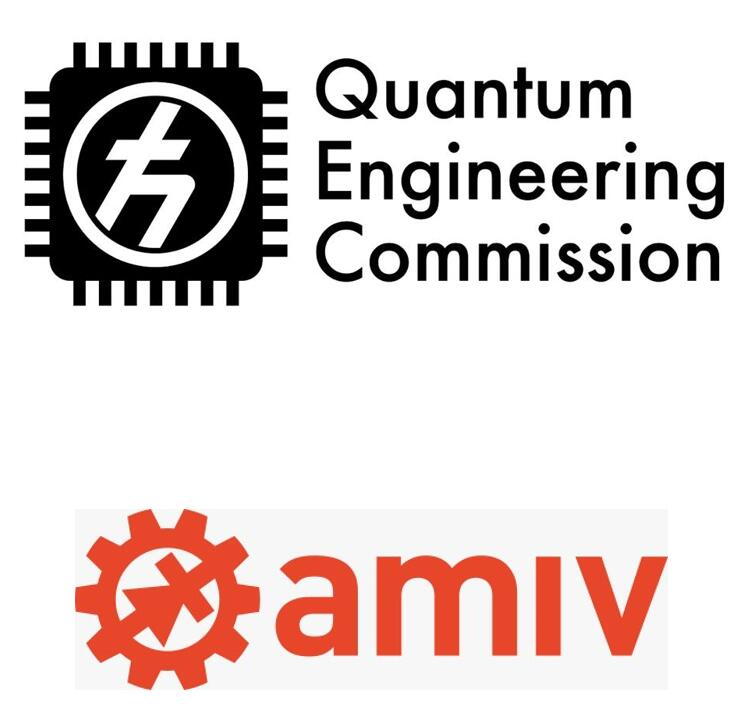
\includegraphics[width=1cm]{2023_04_QEC.png}}, angle=45, opacity=0.3}%
%
\begin{document}%
\normalsize%
\begin{enumerate}%
\item%
He does not let you choose a topic%
\item%
I had the exam this morning, here is how it went:%
\item%
He started by asking how we arrive at the Jaynes{-}Cummings Hamiltonian from the minimal coupling Hamiltonian. He asked about the LWA, then we moved on to the eigenstates of JC. He then asked me about the Purcell regime (what are the relevant parameters), how the spectrum of JC changes in the Purcell regime (no clue), and how it affects the correlation function. He kept asking questions related to the Purcell regime but I had no idea so he changed the topic. %
\item%
We moved on to ion trapping, why in that case the dipole approximation is still valid and what are the relevant physical quantities. %
\item%
He also asked me a few questions about Rabi oscillations and collapse and revival.%
\item%
I had very similar topics to this%
\item%
I would say it very important that you know all assumptions in each regime very well and especially know how to explain them%
\item%
I would also say he does not give you a lot of hints when you are stuck so if you are stuck try saying things that you might think are related because then he will tell you if they are%
\item%
At least that was my experience%
\item%
He asked me to talk about JC and Tavis{-}Cummings, and the differences between them. He wanted to know how we can differentiate whether there is one or many atoms in the cavity by analyzing the leakage (g2 is apparently not the answer he was looking for, I got stuck there for 15min and he didn't wanna move on for some reason, then he revealed the solution but I didn't understand it ). Then he asked about the Purcell regime, he especially wanted to hear the term "large cooperativity". In the end he wanted to know how an two atoms in the dark superpos state can decay and how this depends on the distance between the atoms. I had no clue, then he gave the "hint" that I should consider the wavelength of the e<{-}>g transition which didn't help. He then revealed the…%
\item%
I also had a similar experience.. was asked about JC and it’s approximations in detail. What is important in JC and why do we consider it. I said about Rabi oscillations … and then went on to collapse and revival. He wanted me to tell him what happens if we increase the photons in the cavity and how it affects the revival and collapse time. %
\item%
Also talked a bit about Tavis Cummings. %
\item%
And then at the end about dressed states, why we have antibunching and why we don’t have it when we only have a cavity (without emitter). %
\item%
He also asked many times why are these things important for someone who is not in the quantum optics domain … I am not sure what he expected for an answer …%
\item%
Mine was mostly about Spontaneous Emission both with Wigner Weisskopf and density matrices. He wanted to know the approximation in both cases (Markov Born Reservoir). Then we talked about OBEs in steady state and why you don’t see rabi oscillations there (didn’t fully understand this). Finally we spoke about rabi oscillations in G2%
\item%
For the ones who still have QO, here are my topics: Atac asked me to talk 5 minutes about different ways to couple a laser to the center of mass motion and collective motion of matter. After seeing me severely struggle for 5 min, he had some mercy and asked me to derive the JC Hamiltonian from the minimal coupling Hamiltonian and explain all assumptions \& approximations. That went very well. Then he again asked if with that Hamiltonian I can couple to the center of mass motion of an atom or what other term I need. Again, no idea. In the end he gave me the following exercise which we discussed together:%
\item%
I also did QO this morning: Atac started with same question and I talked a bit about cavity optomechanics and here he asked if the mirror should be heavy or not have a large coupling rate. Then he moved on to trapped ions, because this was what he wanted hear, (he said something that using cavity optomechanics to cool down isn't really used), and here I struggled a bit more. Then he moved on to the exercise%
\item%
He wanted me to explain what each term represents and how this affects the results in the HBT experiment, I had no clue what would be the effect of Gamma1 and he didn't give me the answer so this remains a mystery to me%
\item%
Not sure if it's gonna help much by now, but this is what Atac asked me this morning:%
\item%
First he made me talk for 5 min ish about photon photon interactions.%
\item%
Then he wanted to know if and under which conditions we can have Rabi oscillations between ground state and |{-}, 1> state of JC model driving a cavity in the photon blockade regime.%
\item%
And then he moved to an exercise%
\item%
This was more or less what he showed me (there s a cavity that can lose photons also through a 2 photon process to a reservoir)%
\item%
He wanted me to write a master eq for the system, and then he asked me what would be the output in a HBT setup.%
\item%
Finally (since the answer was antibunching) he asked if we could have HOM interference between the photons emitted by two such cavities, which I couldn't answer (and he didn't give me the answer either...)%
\item%
I was right after him and he started with this same topic.%
\item%
Then he asked me about hom interferometer (everything about it). I talked also about bell basis and he asked me about the shape of photon pulses (what’s the width and what happens if we have two distant emitters)%
\end{enumerate}%
\end{document}